\documentclass{article}
\usepackage{graphicx} % Required for inserting images
\usepackage{float}

\title{Optimization Methods PS s7 Lab 1}
\author{Joris Plaščinskas}
\date{September 2024}


\begin{document}
    \maketitle
    \section{One Dimension Optimization}
        The goal of this laboratory work is to get familiar with one dimensional optimization methods. I will try to minimize this 4th degree polynomial function: $(\frac{(x^{2} - a)^{2}}{b}) - 1$. In my case: $a=2,b=2$, because my student number is 2016020. I will use 3 different optimization methods and try to compare them in the end.
    \section{Interval Split Method}
        I chose to use 3-point interval split method. The algorithm relies on 5 points: left bound, right bound, left x, middle x, right x. Each iteration the interval is split into 4 equal parts: $I-x_1-x_m-x_2-r$ - here I/r are the left/right bounds. At the start of each iteration $f(x_1), f(x_m), f(x_2)$ are calculated. The algorithm then branches out:
        \begin{itemize}
            \item If $f(x_1) < f(x_m)$, then $r=x_m$.
            \item If $f(x_2) < f(x_m)$, then $I=x_m$.
            \item Else ($f(x_1) \geq f(x_m)$ and $f(x_2) \geq f(x_m)$), then $I=x_1$ and $r=x_2$.
        \end{itemize}
        The algorithm is slightly optimized by recycling the $x_1$ or $x_2$ and assigning them to $x_m$ after each iteration.
        \subsection*{Results}
            \begin{figure}[H]
                \centering
                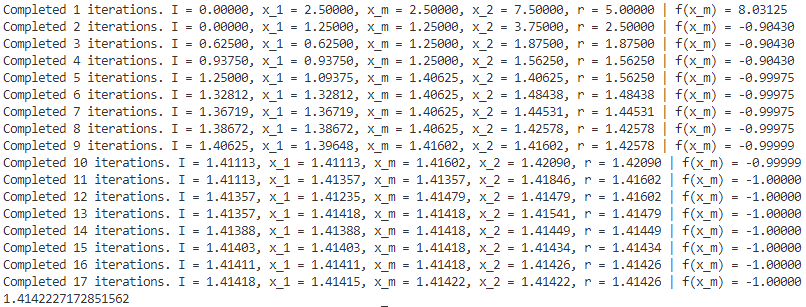
\includegraphics[width=1\textwidth]{interval.png}
                \caption{Interval split results}
                \label{fig:ml}
            \end{figure}
    \section{Golden Ratio Search Method}
        Golden Ratio Search is in principal also an interval split method and is very similar to the previous method. The main difference is that the interval is only split at 2 points and the points are placed at specifically $L * 0.618...$ away from the boundaries, so that they can be recycled after each iteration.
        \subsection*{Results}
            \begin{figure}[H]
                \centering
                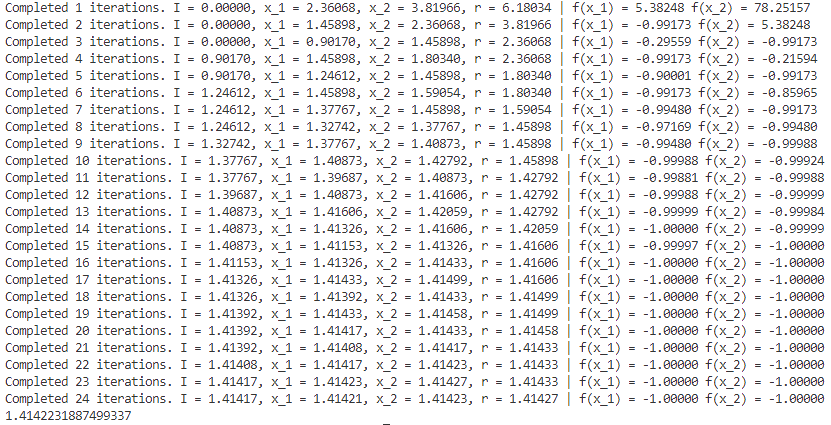
\includegraphics[width=1\textwidth]{golden-ratio.png}
                \caption{Golden ratio search results}
                \label{fig:ml}
            \end{figure}
    \section{Newton's Method}
        Newton's Method for finding 0's of a function has two steps: on  and then trying to reach 0 of that linear function. Using Newton's Method for optimization is very similar, it
        \begin{itemize}
            \item Making a linear approximation of that function at any random $x \in [I,r]$.
            \item Setting x to the $y=0$ value of that linear approximation and repeating with the new x until step size becomes acceptably small.
        \end{itemize}
        \subsection*{Results}
            \begin{figure}[H]
                \centering
                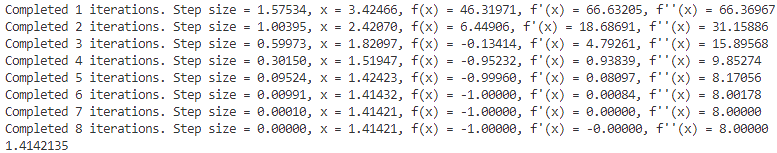
\includegraphics[width=1\textwidth]{newton.png}
                \caption{Newton's results}
                \label{fig:ml}
            \end{figure}
    \section{Comparison}
        All functions managed to reached the same minimum (when rounded to 4th decimal place). The key differences were: iteration count, computations count and code length. Newton's method was around 3 times shorter to code, compared to the other two methods. The count of computing the objective function is the same as iterations count in the Golden Ratio Search method and double the iterations count in Newton's and Interval method's (note: in Newton's method you are computing the first and second derivatives of the objective function, but not the objective function it's self).
        \begin{table}[h!]
            \centering
            \begin{tabular}{|c|c|c|c|}
            \hline
            & Interval & Golden 2 & Newton's \\
            \hline
            Iterations & 17 & 24 & 8 \\
            \hline
            Computations& 34 & 24 & 16 \\
            \hline
            \end{tabular}
            \caption{Final results}
        \end{table}
    \section{Plots}
        \begin{figure}[H]
            \centering
            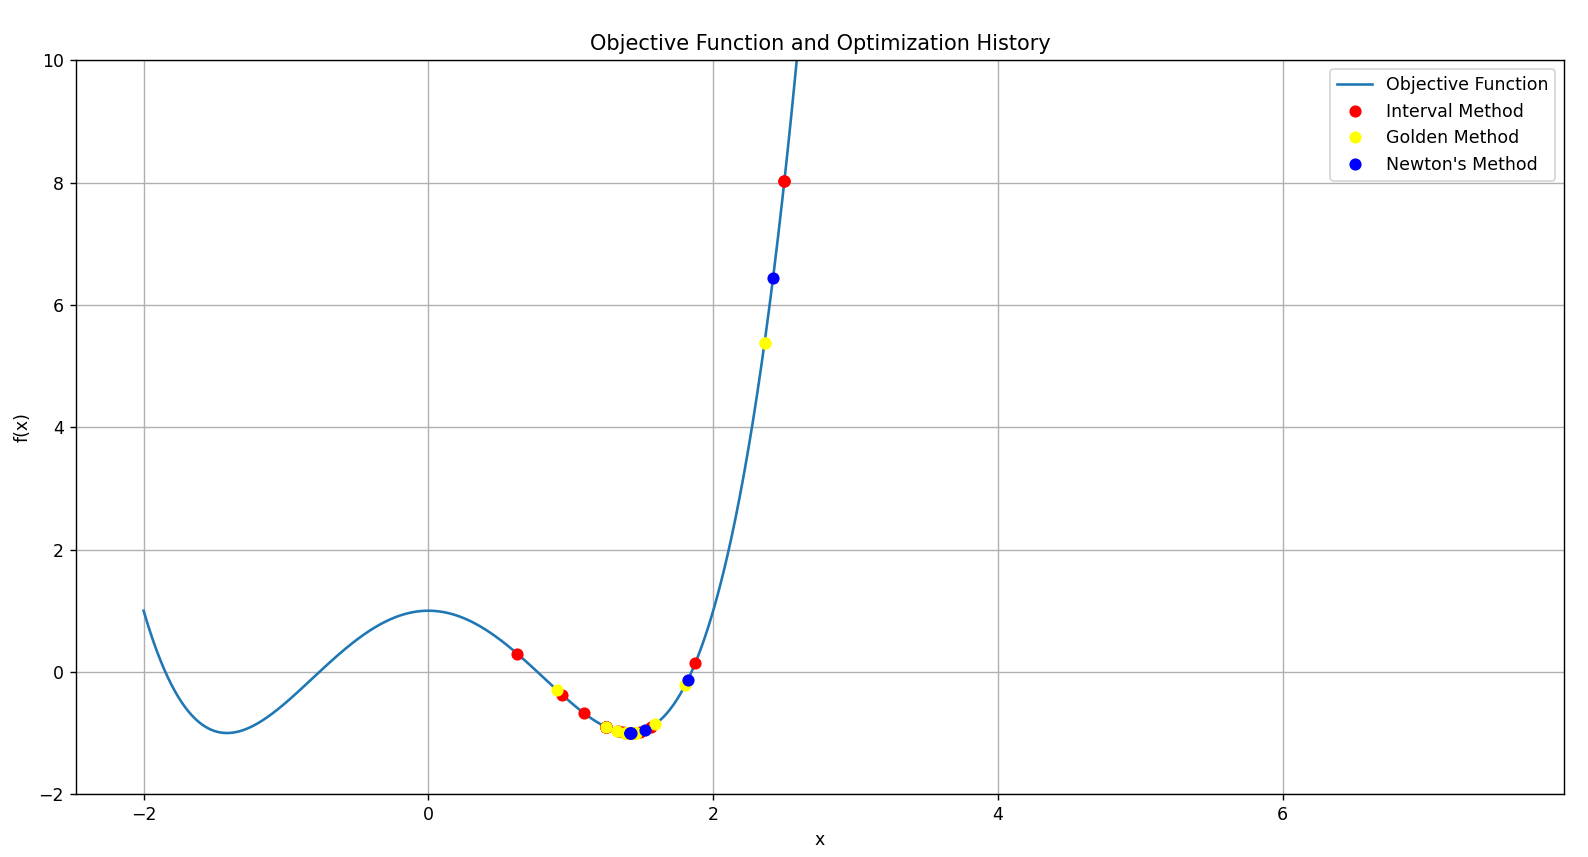
\includegraphics[width=1\textwidth]{plot-1.png}
            \caption{Objective function and optimization history plot}
            \label{fig:zoomed-out}
        \end{figure}
        \begin{figure}[H]
            \centering
            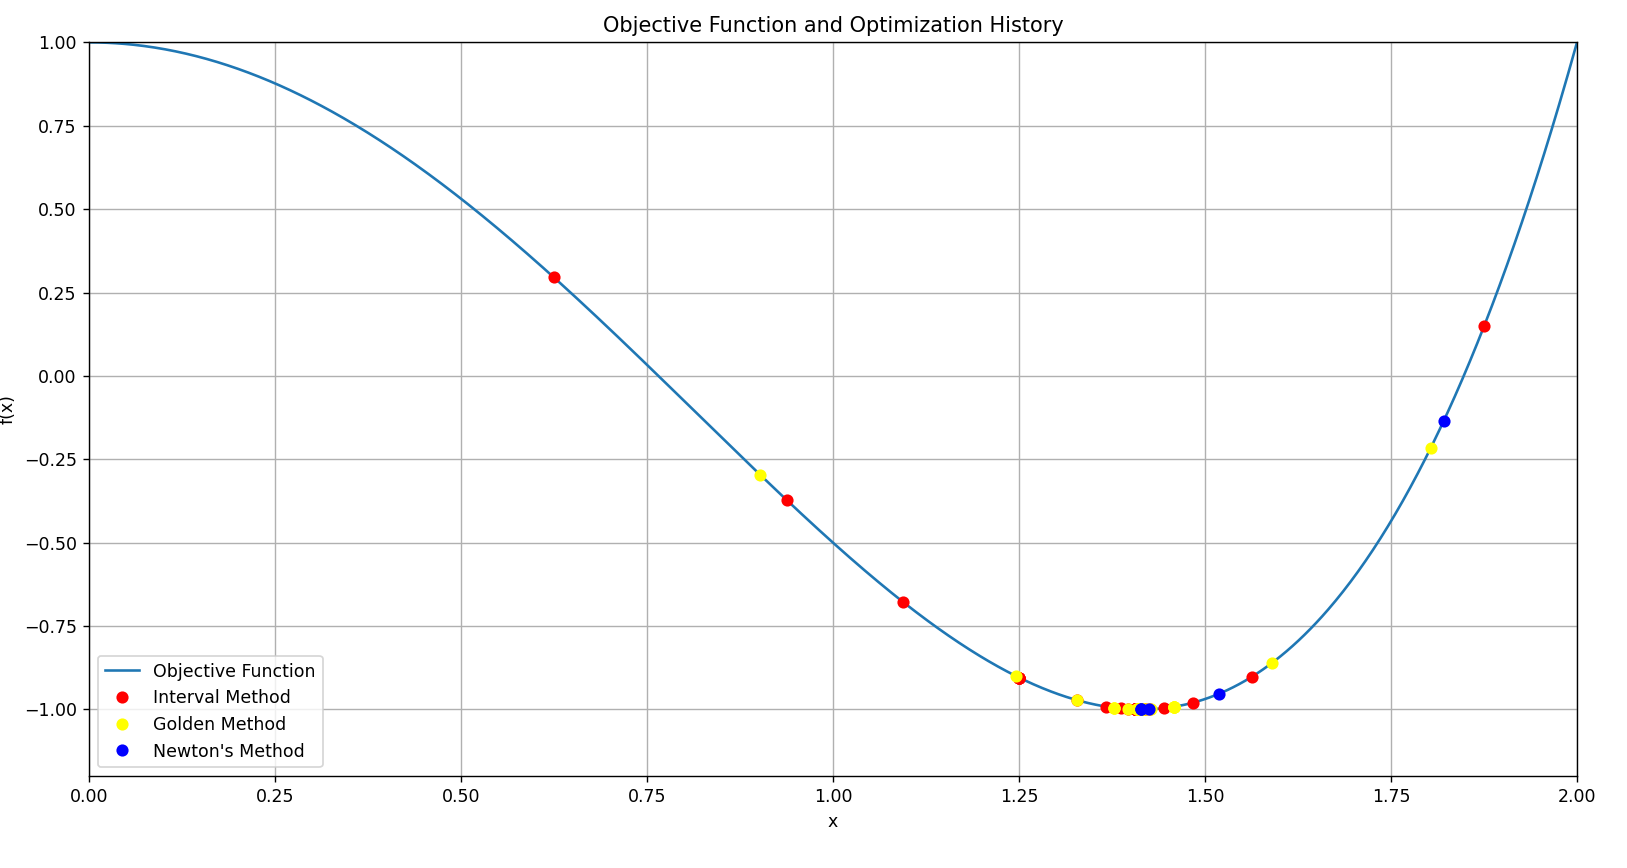
\includegraphics[width=1\textwidth]{plot-2.png}
            \caption{Zoomed in on Figure \ref{fig:zoomed-out}}
            \label{fig:zommed-in}
        \end{figure}
\end{document}
